\pdfminorversion=4
\documentclass[aspectratio=169]{beamer}

\mode<presentation>
{
  \usetheme{default}
  \usecolortheme{default}
  \usefonttheme{default}
  \setbeamertemplate{navigation symbols}{}
  \setbeamertemplate{caption}[numbered]
  \setbeamertemplate{footline}[frame number]  % or "page number"
  \setbeamercolor{frametitle}{fg=white}
  \setbeamercolor{footline}{fg=black}
} 

\usepackage[english]{babel}
\usepackage[utf8x]{inputenc}
\usepackage{tikz}
\usepackage{courier}
\usepackage{array}
\usepackage{bold-extra}
\usepackage{minted}
\usepackage[thicklines]{cancel}
\usepackage{fancyvrb}

\xdefinecolor{dianablue}{rgb}{0.18,0.24,0.31}
\xdefinecolor{darkblue}{rgb}{0.1,0.1,0.7}
\xdefinecolor{darkgreen}{rgb}{0,0.5,0}
\xdefinecolor{darkgrey}{rgb}{0.35,0.35,0.35}
\xdefinecolor{darkorange}{rgb}{0.8,0.5,0}
\xdefinecolor{darkred}{rgb}{0.7,0,0}
\definecolor{darkgreen}{rgb}{0,0.6,0}
\definecolor{mauve}{rgb}{0.58,0,0.82}

\title[2019-10-03-yana-david]{Conversation with Yana and David about Awkward 1.0}
\author{Jim Pivarski}
\institute{Princeton University -- IRIS-HEP}
\date{October 3, 2019}

\usetikzlibrary{shapes.callouts}

\begin{document}

\logo{\pgfputat{\pgfxy(0.11, 7.4)}{\pgfbox[right,base]{\tikz{\filldraw[fill=dianablue, draw=none] (0 cm, 0 cm) rectangle (50 cm, 1 cm);}\mbox{\hspace{-8 cm}
\includegraphics[height=1 cm]{princeton-logo-long.png}\hspace{0.1 cm}\raisebox{0.1 cm}{
\includegraphics[height=0.8 cm]{iris-hep-logo-long.png}}\hspace{0.1 cm}}}}}

\begin{frame}
  \titlepage
\end{frame}

\logo{\pgfputat{\pgfxy(0.11, 7.4)}{\pgfbox[right,base]{\tikz{\filldraw[fill=dianablue, draw=none] (0 cm, 0 cm) rectangle (50 cm, 1 cm);}\mbox{\hspace{-8 cm}
\includegraphics[height=1 cm]{princeton-logo.png}\hspace{0.1 cm}\raisebox{0.1 cm}{
\includegraphics[height=0.8 cm]{iris-hep-logo.png}}\hspace{0.1 cm}}}}}

% Uncomment these lines for an automatically generated outline.
%\begin{frame}{Outline}
%  \tableofcontents
%\end{frame}

% START START START START START START START START START START START START START

\begin{frame}{Context: columnar data analysis}
\large
\vspace{0.5 cm}
\begin{columns}
\column{1.1\linewidth}
\begin{itemize}\setlength{\itemsep}{1 cm}
\item \textcolor{darkblue}{\Large uproot}: reads columnar data (``split'' in ROOT terminology) from ROOT files without reconstructing objects---leaving them as arrays or jagged arrays.

\vspace{0.25 cm}
\textcolor{gray}{\normalsize (used by CMS, ATLAS, LHCb, NOvA, nuclear physics, theory, and gamma-ray astronomy)}

\item \textcolor{darkblue}{\Large awkward-array}: presents columnar data as though they were arrays of objects.

\vspace{0.25 cm}
\textcolor{gray}{\normalsize (used by 41 other projects on GitHub, including uproot and Coffea)}

\item \textcolor{darkblue}{\Large Coffea}: more fully featured data analysis package, developed by Fermilab physicists.

\vspace{0.25 cm}
\textcolor{gray}{\normalsize (used by at least 8 CMS analyses)}
\end{itemize}
\end{columns}
\end{frame}

\begin{frame}{Columnar data structures}
\vspace{0.2 cm}
\begin{center}
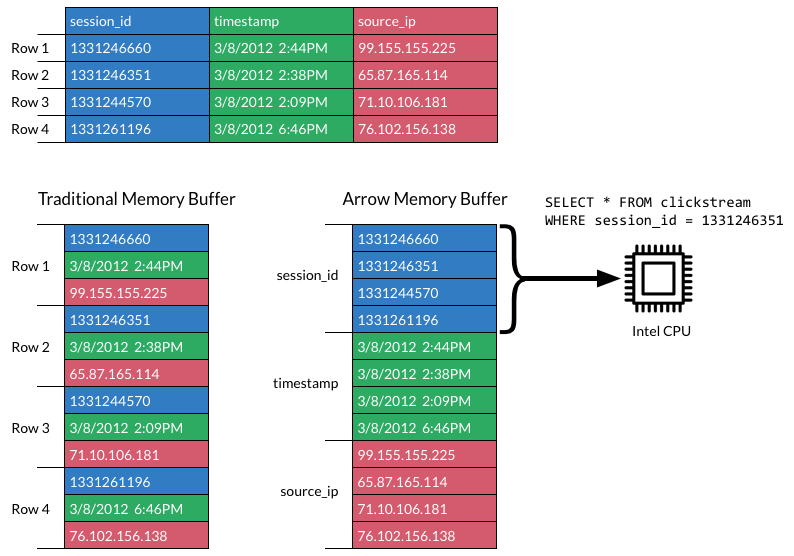
\includegraphics[width=0.7\linewidth]{simd.png}
\end{center}

Source: \textcolor{blue}{\url{http://arrow.apache.org}}
\end{frame}

\begin{frame}{Columnar data structures}
\begin{center}
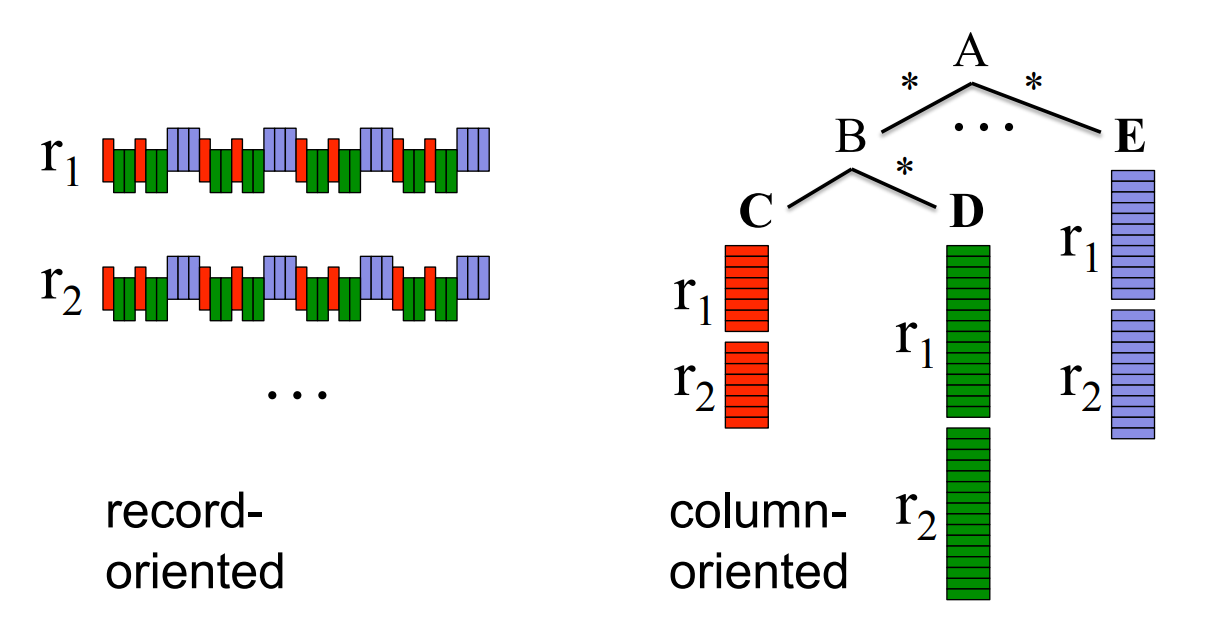
\includegraphics[width=0.95\linewidth]{google-dremel-fig1.png}
\end{center}

Source: \textcolor{blue}{\url{https://ai.google/research/pubs/pub36632}}
\end{frame}

\begin{frame}[fragile]{Columnar data structures}
\vspace{0.5 cm}
\begin{columns}
\column{0.5\linewidth}
\small
\begin{Verbatim}[commandchars=\\\{\}]
[[Muon(\textcolor{darkgreen}{31.1}, \textcolor{darkorange}{-0.481}, \textcolor{blue}{0.882}),
      Muon(\textcolor{darkgreen}{9.76}, \textcolor{darkorange}{-0.124}, \textcolor{blue}{0.924}),
      Muon(\textcolor{darkgreen}{8.18}, \textcolor{darkorange}{-0.119}, \textcolor{blue}{0.923})],
 [Muon(\textcolor{darkgreen}{5.27}, \textcolor{darkorange}{1.246}, \textcolor{blue}{-0.991})],
 [Muon(\textcolor{darkgreen}{4.72}, \textcolor{darkorange}{-0.207}, \textcolor{blue}{0.953})],
 [Muon(\textcolor{darkgreen}{8.59}, \textcolor{darkorange}{-1.754}, \textcolor{blue}{-0.264}),
      Muon(\textcolor{darkgreen}{8.714}, \textcolor{darkorange}{0.185}, \textcolor{blue}{0.629})]
]
\end{Verbatim}
\column{0.35\linewidth}
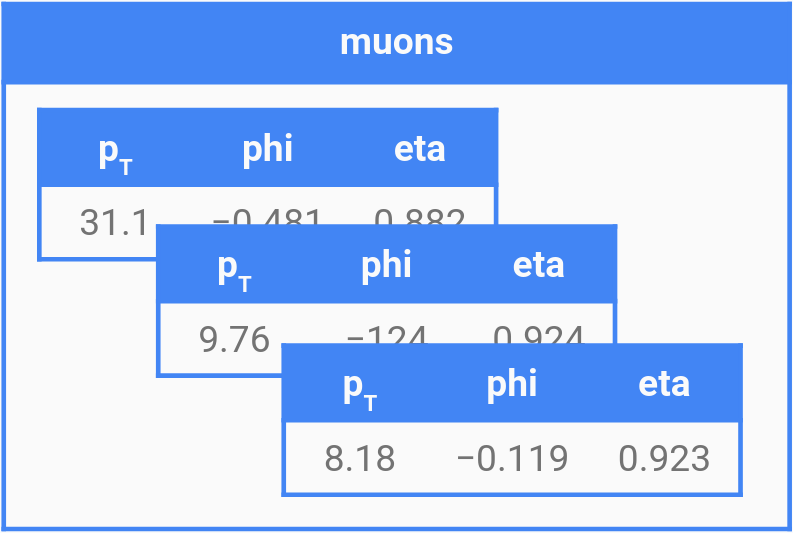
\includegraphics[width=\linewidth]{muons-as-objects.png}
\end{columns}
\vspace{0.5 cm}
\large The trick: represent structure with \only<1>{\textcolor{red}{counts}}\only<2,3,4>{counts} or \only<2>{\textcolor{red}{offsets}}\only<1,3,4>{offsets} or \only<3>{\textcolor{red}{starts/stops}}\only<1,2,4>{starts/stops} or \only<4>{\textcolor{red}{parents}}\only<1,2,3>{parents}.
\vspace{0.25 cm}
\begin{tabular}{r l}
\only<1>{\small \textcolor{red}{counts}  & \textcolor{red}{\tt\scriptsize \ \ \ \ \ 3,\ \ \ \ \ \ \ \ \ \ \ \ \ \ \ \ \ \ \ \ \ \ 1,\ \ \ \ \ \ 1,\ \ \ \ \ \ 2\ \ \ \ \ \ \ \ \ } \\}
\only<2>{\small \textcolor{red}{offsets} & \textcolor{red}{\tt\scriptsize \ \ \ \ \ 0,\ \ \ \ \ \ \ \ \ \ \ \ \ \ \ \ \ \ \ \ \ \ 3,\ \ \ \ \ \ 4,\ \ \ \ \ \ 5,\ \ \ \ \ \ \ 7} \\}
\only<4>{\small \textcolor{red}{parents} & \textcolor{red}{\tt\scriptsize \ \ \ \ \ 0,\ \ \ \ \ \ 0,\ \ \ \ \ \ 0,\ \ \ \ \ \ 1,\ \ \ \ \ \ 2,\ \ \ \ \ \ 3,\ \ \ \ \ 3} \\}
\only<3>{\small \textcolor{red}{starts}  & \textcolor{red}{\tt\scriptsize \ \ \ \ \ 0,\ \ \ \ \ \ \ \ \ \ \ \ \ \ \ \ \ \ \ \ \ \ 3,\ \ \ \ \ \ 4,\ \ \ \ \ \ 5\ \ \ \ \ \ \ \ \ } \\}
\uncover<3>{\small \textcolor{red}{stops}   & \textcolor{red}{\tt\scriptsize \ \ \ \ \ 3,\ \ \ \ \ \ \ \ \ \ \ \ \ \ \ \ \ \ \ \ \ \ 4,\ \ \ \ \ \ 5,\ \ \ \ \ \ 7\ \ \ \ \ \ \ \ \ } \\}
\small \mbox{\hspace{1 cm}$p_T$} & \textcolor{darkgreen}{\tt\scriptsize \ \ 31.1,\ \ \ 9.76,\ \ \ 8.18,\ \ \ 5.27,\ \ \ 4.72,\ \ \ 8.59, 8.714} \\
\small phi &  \textcolor{darkorange}{\tt\scriptsize -0.481,\ -0.123,\ -0.119,\ \ 1.246,\ -0.207,\ -1.754,\ 0.185} \\
\small eta &        \textcolor{blue}{\tt\scriptsize \ 0.882,\ \ 0.924,\ \ 0.923,\ -0.991,\ \ 0.953,\ -0.264,\ 0.629} \\
\end{tabular}
\end{frame}

\begin{frame}[fragile]{Operating on data in columnar form}
\vspace{0.5 cm}
\textcolor{red}{``Remove the first muon from each event.''} \uncover<2->{\textcolor{red}{\bf$\longrightarrow$ rewrite all inner lists.}}
\scriptsize
\begin{onlyenv}<1>
\begin{Verbatim}[commandchars=\\\{\}]
[[Muon(\textcolor{darkgreen}{31.1}, \textcolor{darkorange}{-0.481}, \textcolor{blue}{0.882}), Muon(\textcolor{darkgreen}{9.76}, \textcolor{darkorange}{-0.124}, \textcolor{blue}{0.924}), Muon(\textcolor{darkgreen}{8.18}, \textcolor{darkorange}{-0.119}, \textcolor{blue}{0.923})],
 [Muon(\textcolor{darkgreen}{5.27}, \textcolor{darkorange}{1.246}, \textcolor{blue}{-0.991})],
 [Muon(\textcolor{darkgreen}{4.72}, \textcolor{darkorange}{-0.207}, \textcolor{blue}{0.953})],
 [Muon(\textcolor{darkgreen}{8.59}, \textcolor{darkorange}{-1.754}, \textcolor{blue}{-0.264}), Muon(\textcolor{darkgreen}{8.714}, \textcolor{darkorange}{0.185}, \textcolor{blue}{0.629})],
 ...
\end{Verbatim}
\end{onlyenv}\begin{onlyenv}<2->
\begin{Verbatim}[commandchars=\\\{\}]
[[     \textcolor{darkgreen}{    }  \textcolor{darkorange}{      }  \textcolor{blue}{     }   Muon(\textcolor{darkgreen}{9.76}, \textcolor{darkorange}{-0.124}, \textcolor{blue}{0.924}), Muon(\textcolor{darkgreen}{8.18}, \textcolor{darkorange}{-0.119}, \textcolor{blue}{0.923})],
 [     \textcolor{darkgreen}{    }  \textcolor{darkorange}{     }  \textcolor{blue}{      } ],
 [     \textcolor{darkgreen}{    }  \textcolor{darkorange}{      }  \textcolor{blue}{     } ],
 [     \textcolor{darkgreen}{    }  \textcolor{darkorange}{      }  \textcolor{blue}{      }   Muon(\textcolor{darkgreen}{8.714}, \textcolor{darkorange}{0.185}, \textcolor{blue}{0.629})],
 ...
\end{Verbatim}
\end{onlyenv}
\normalsize
\vspace{0.5 cm}
\textcolor{red}{``Remove the first muon from each event.''} \uncover<2->{\textcolor{red}{\bf$\longrightarrow$ increase all starts by 1.}}
\vspace{0.25 cm}
\begin{onlyenv}<1>
\begin{tabular}{r l}
\small starts  &                    {\tt\scriptsize \ \ \ \ \ 0,\ \ \ \ \ \ \ \ \ \ \ \ \ \ \ \ \ \ \ \ \ \ 3,\ \ \ \ \ \ 4,\ \ \ \ \ \ 5\ \ \ \ \ \ \ \ \ } \\
\small stops   &                    {\tt\scriptsize \ \ \ \ \ 3,\ \ \ \ \ \ \ \ \ \ \ \ \ \ \ \ \ \ \ \ \ \ 4,\ \ \ \ \ \ 5,\ \ \ \ \ \ 7\ \ \ \ \ \ \ \ \ } \\
\small $p_T$ & \textcolor{darkgreen}{\tt\scriptsize \ \ 31.1,\ \ \ 9.76,\ \ \ 8.18,\ \ \ 5.27,\ \ \ 4.72,\ \ \ 8.59, 8.714} \\
\small phi &  \textcolor{darkorange}{\tt\scriptsize -0.481,\ -0.123,\ -0.119,\ \ 1.246,\ -0.207,\ -1.754,\ 0.185} \\
\small eta &        \textcolor{blue}{\tt\scriptsize \ 0.882,\ \ 0.924,\ \ 0.923,\ -0.991,\ \ 0.953,\ -0.264,\ 0.629} \\
\end{tabular}
\end{onlyenv}\begin{onlyenv}<2->
\begin{tabular}{r l}
\small starts  &     \textcolor{red}{\tt\scriptsize \ \ \ \ \ 1,\ \ \ \ \ \ \ \ \ \ \ \ \ \ \ \ \ \ \ \ \ \ 4,\ \ \ \ \ \ 5,\ \ \ \ \ \ 6\ \ \ \ \ \ \ \ \ } \\
\small stops   &                    {\tt\scriptsize \ \ \ \ \ 3,\ \ \ \ \ \ \ \ \ \ \ \ \ \ \ \ \ \ \ \ \ \ 4,\ \ \ \ \ \ 5,\ \ \ \ \ \ 7\ \ \ \ \ \ \ \ \ } \\
\small $p_T$ & \textcolor{darkgreen}{\tt\scriptsize \ \ 31.1,\ \ \ 9.76,\ \ \ 8.18,\ \ \ 5.27,\ \ \ 4.72,\ \ \ 8.59, 8.714} \\
\small phi &  \textcolor{darkorange}{\tt\scriptsize -0.481,\ -0.123,\ -0.119,\ \ 1.246,\ -0.207,\ -1.754,\ 0.185} \\
\small eta &        \textcolor{blue}{\tt\scriptsize \ 0.882,\ \ 0.924,\ \ 0.923,\ -0.991,\ \ 0.953,\ -0.264,\ 0.629} \\
\end{tabular}\end{onlyenv}
\vspace{0.25 cm}

\large
\vspace{0.2 cm}
\uncover<2>{We didn't need to touch any contents (i.e.\ read from disk/decompress them).}
\end{frame}

\begin{frame}{On Scientific Linux, uproot/awkward is installed as often as Pandas}
\vspace{0.5 cm}
\begin{columns}
\column{1.2\linewidth}
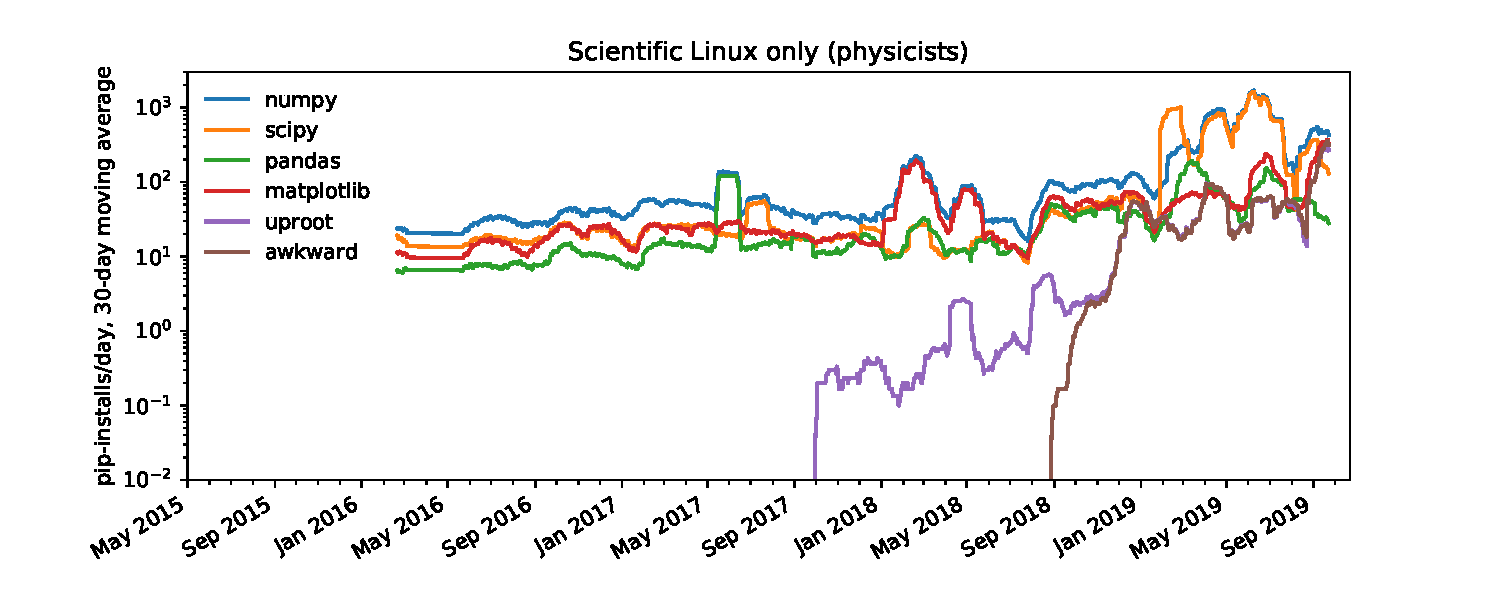
\includegraphics[width=\linewidth]{pip-scilinux-uproot.pdf}
\end{columns}
\end{frame}

\begin{frame}{And so is Coffea (very recently)\ldots}
\vspace{0.5 cm}
\begin{columns}
\column{1.2\linewidth}
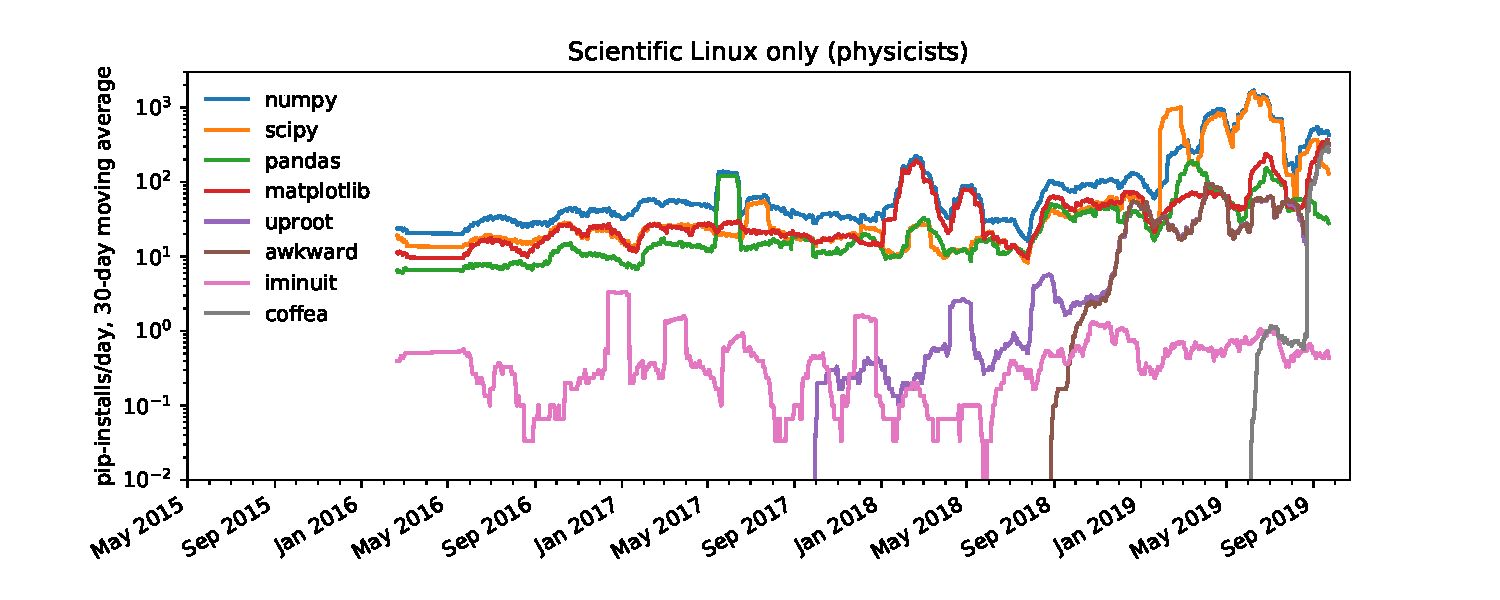
\includegraphics[width=\linewidth]{pip-scilinux-uproot-iminuit.pdf}
\end{columns}
\end{frame}

\begin{frame}{\ldots more so than deep learning libraries (TensorFlow and Torch)}
\vspace{0.5 cm}
\begin{columns}
\column{1.2\linewidth}
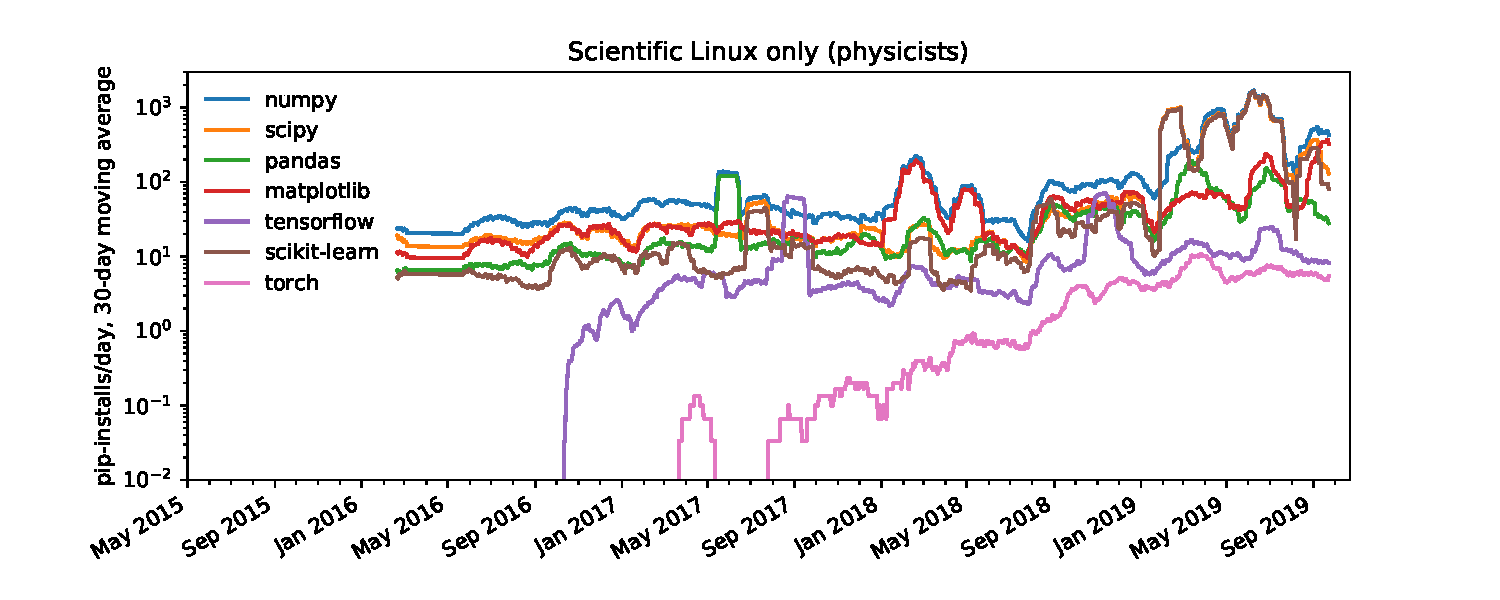
\includegraphics[width=\linewidth]{pip-scilinux-ml.pdf}
\end{columns}
\end{frame}

\begin{frame}{(Though in general, uproot is 4 orders of magnitude below Pandas)}
\vspace{0.5 cm}
\begin{columns}
\column{1.2\linewidth}
\only<1>{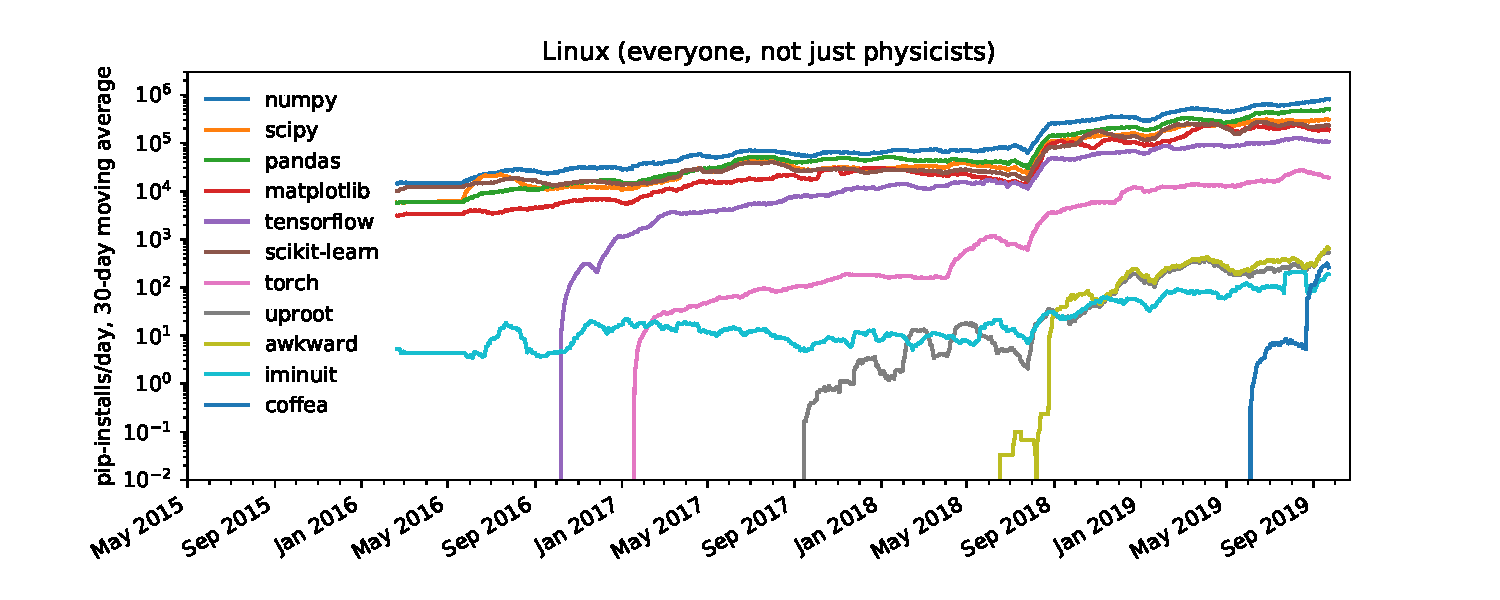
\includegraphics[width=\linewidth]{pip-linux.pdf}}\only<2>{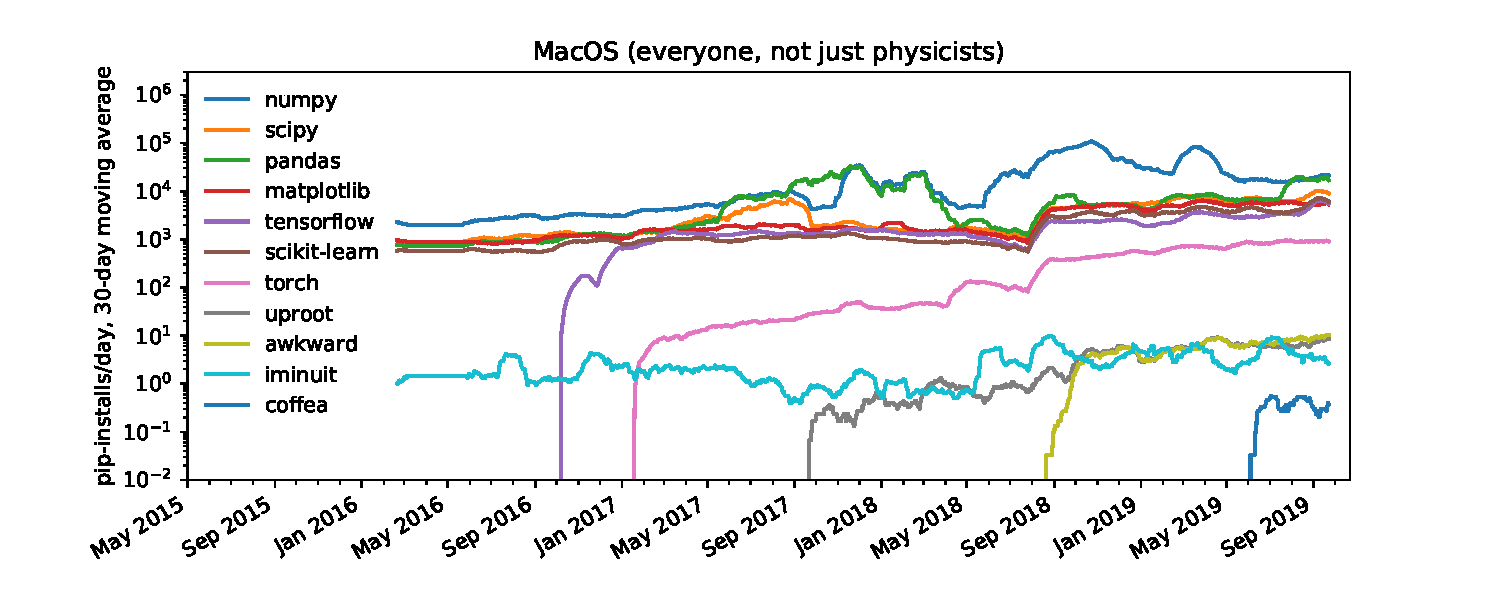
\includegraphics[width=\linewidth]{pip-macos.pdf}}\only<3>{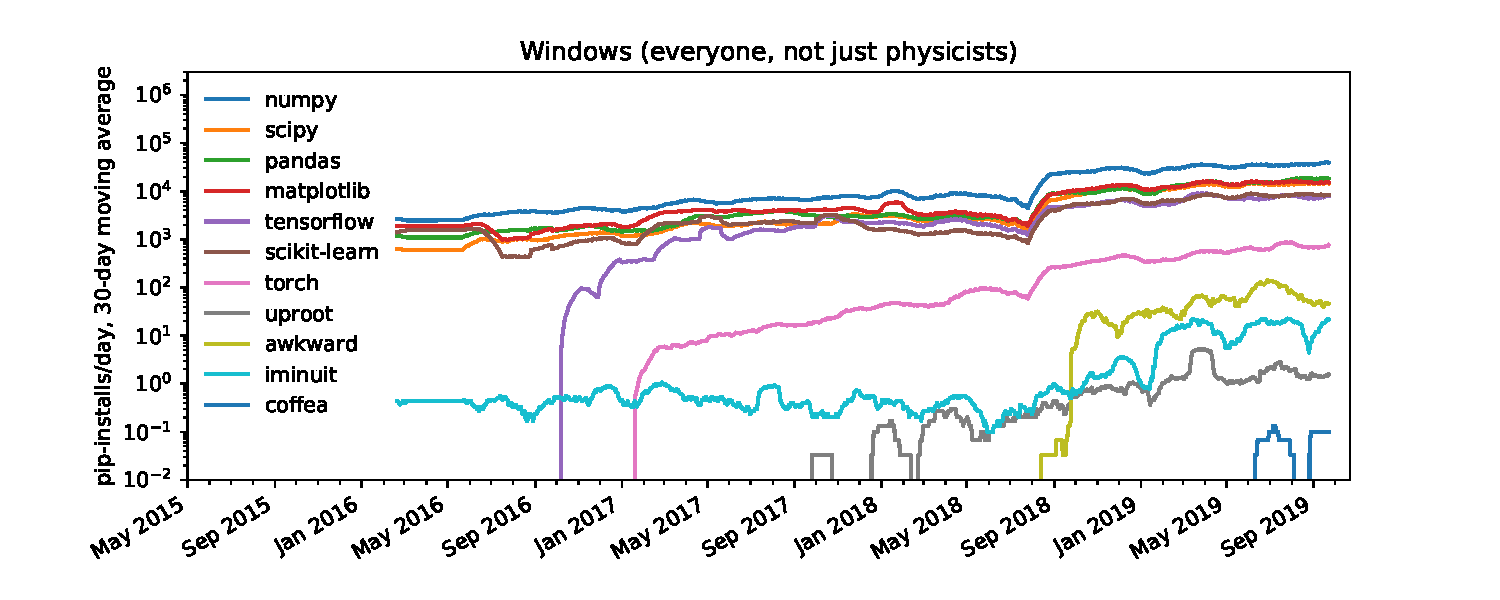
\includegraphics[width=\linewidth]{pip-windows.pdf}}
\end{columns}
\end{frame}

\begin{frame}{Uproot/Awkward maintainance is pretty much constant}
\Large
\vspace{0.75 cm}
\begin{columns}
\column{0.36\linewidth}
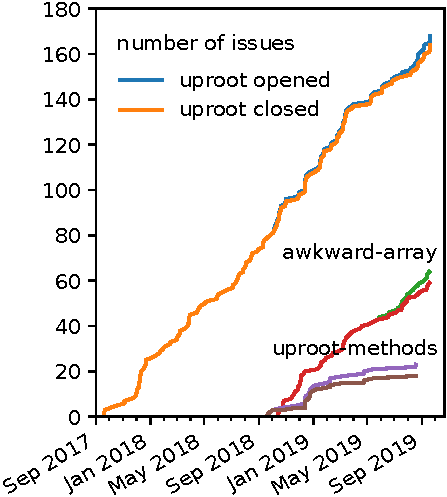
\includegraphics[width=\linewidth]{uproot-issues.pdf}

\column{0.72\linewidth}
\only<1>{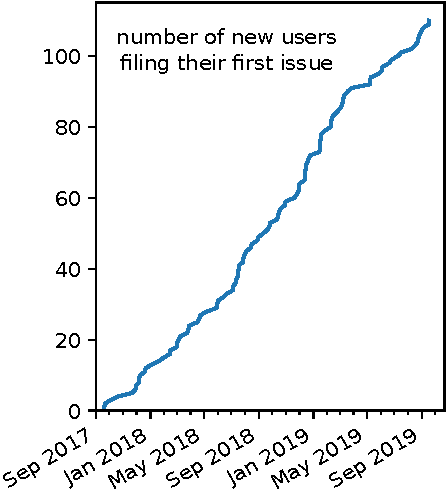
\includegraphics[width=0.5\linewidth]{uproot-users.pdf}\hfill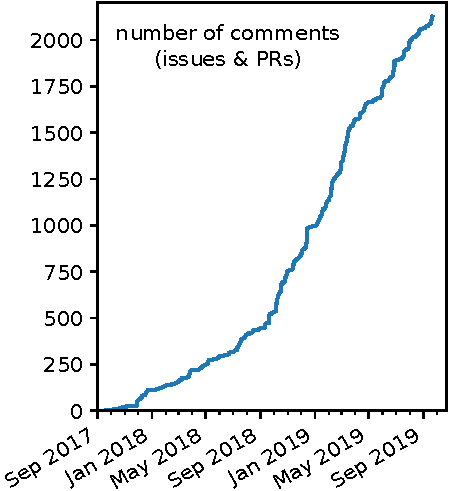
\includegraphics[width=0.5\linewidth]{uproot-comments.pdf}}\only<2->{\hfill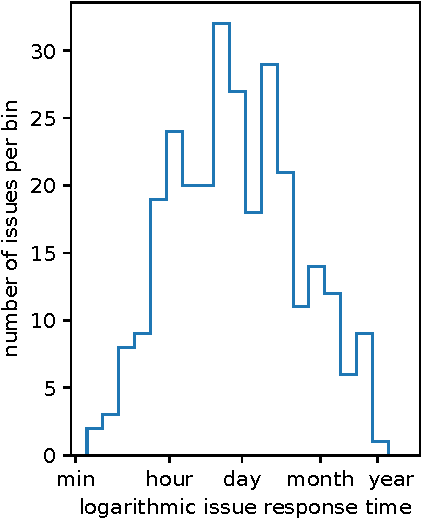
\includegraphics[width=0.45\linewidth]{uproot-response-time.pdf}\hfill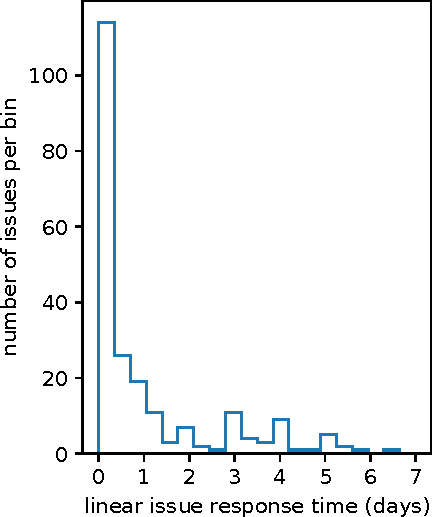
\includegraphics[width=0.45\linewidth]{uproot-response-time-linear.pdf}}
\end{columns}
\end{frame}

\begin{frame}{Moving forward}
\large
\vspace{0.5 cm}
\begin{itemize}\setlength{\itemsep}{0.75 cm}
\item Uproot has been in use for 2 years now and is fine as-is. Maintenance with no major developments \textcolor{gray}{(apart from Pratyush's TTree-writing project)}.

\item Awkward has been in use for 1 year now, and there are

\vspace{0.2 cm}
\begin{itemize}\setlength{\itemsep}{0.2 cm}
\item \large \textcolor{darkblue}{structural issues:} hard to keep interface consistent across all data types
\item \large \textcolor{darkblue}{interface issues:} some visible features are confusing to users; need a semi-private between private and public.
\end{itemize}

\vspace{0.2 cm}
More detailed breakdown in this Google Doc (click): \normalsize

\vspace{0.2 cm}
\textcolor{blue}{\url{https://docs.google.com/document/d/1lj8ARTKV1_hqGTh0W_f01S6SsmpzZAXz9qqqWnEB3j4/edit?usp=sharing}}
\end{itemize}
\end{frame}

\begin{frame}{Awkward 1.0, developed in a separate repo from Awkward 0.x}
\vspace{0.2 cm}
\begin{columns}
\column{1.15\linewidth}
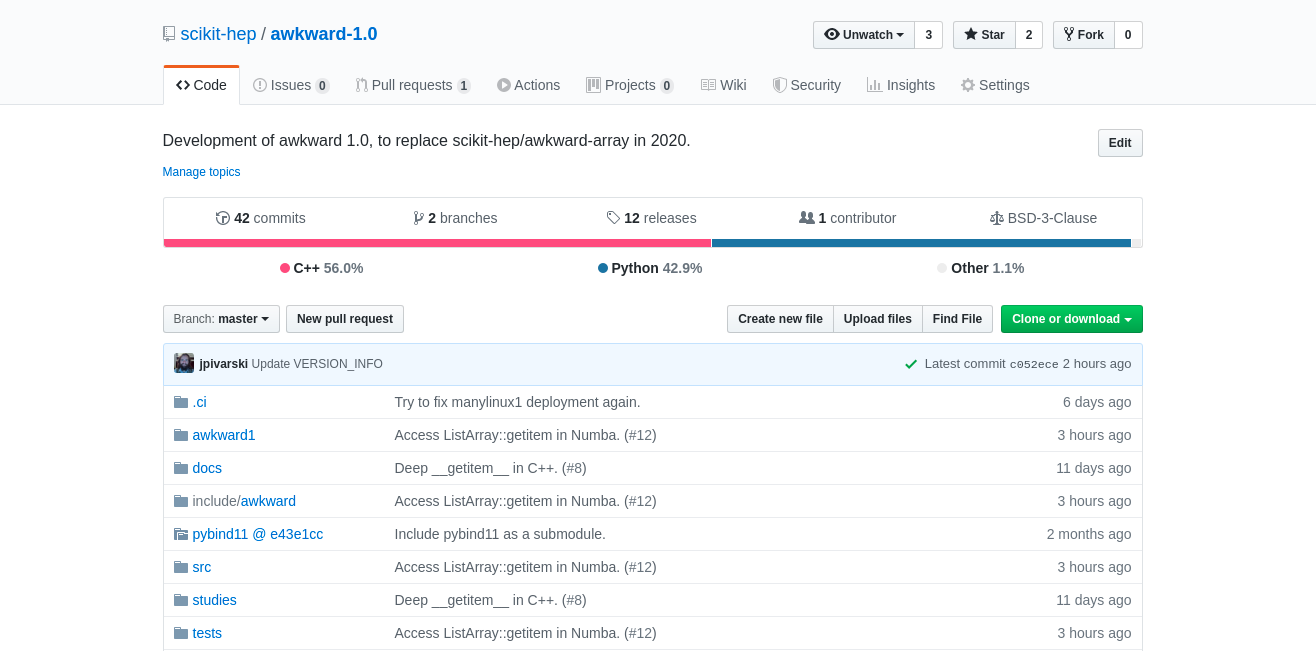
\includegraphics[width=\linewidth]{awkward-1-github.png}
\end{columns}
\end{frame}

\begin{frame}{Architecture of Awkward 1.0}
\large
\vspace{0.5 cm}
\begin{columns}
\column{0.5\linewidth}
\vspace{-0.2 cm}

\textcolor{darkblue}{Layer 1:} Python user interface: a single \mintinline{python}{awkward.Array} class.
\vspace{\baselineskip}

\vspace{0.18 cm}
\textcolor{darkblue}{Layer 2:} Structure classes, ``layout''

(e.g.\ \mintinline{python}{ListArray}/\mintinline{python}{RecordArray}).
\vspace{\baselineskip}

\vspace{0.18 cm}
\textcolor{darkblue}{Layer 3:} Memory management, array allocation and ownership; reference counting.
\vspace{\baselineskip}

\vspace{0.18 cm}
\textcolor{darkblue}{Layer 4:} Implementations, where we write \mintinline{python}{for} loops. The only layer that needs to be optimized.

\column{0.5\linewidth}
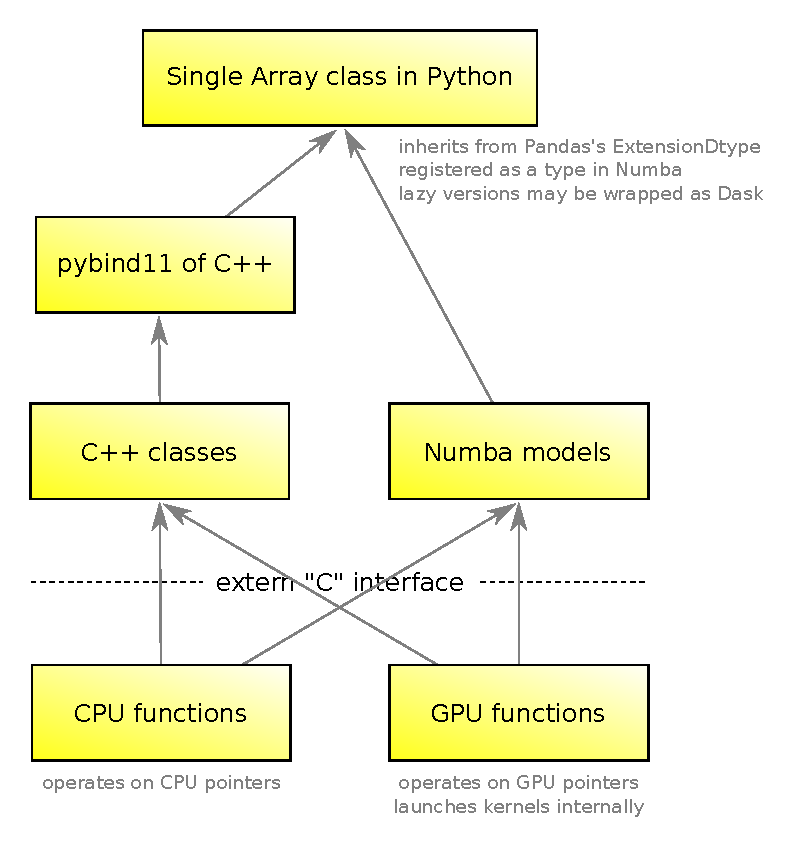
\includegraphics[width=\linewidth]{awkward-1-0-layers.pdf}
\end{columns}
\end{frame}

\begin{frame}{Implications of columnar data representation and processing}
\large
\vspace{0.5 cm}
\begin{itemize}\setlength{\itemsep}{0.6 cm}
\item Length of arrays scale with number of events or particles; number of real C++ or Python objects scales with the complexity of the event type.

\vspace{0.2 cm}
$\rightarrow$ a large dataset ($\sim 10^9$ events) might consist of only 100 C++ objects.

\item Data types must be determined at runtime (for compatibility with Python and ease of handling new data).

\vspace{0.2 cm}
$\rightarrow$ we use \mintinline{c++}{std::shared_ptr}, virtual methods, \mintinline{c++}{dynamic_cast} freely.

\item Layer 3 (C++/Numba) is only concerned with tracking memory ownership and picking the right Layer 4 function to call.

\begin{itemize}
\item \large Layer 3 performs $\mathcal{O}(100)$ steps with slow polymorphism.
\item \large Layer 4 performs $\mathcal{O}(10^9)$ steps in highly optimized loops or GPU kernels.
\end{itemize}
\end{itemize}
\end{frame}

\begin{frame}[fragile]{Example of what layer 4 looks like}
\tiny
\vspace{0.05 cm}
\begin{columns}
\column{1.1\linewidth}
\begin{minted}{c++}
extern "C" {
  Error awkward_listarray32_getitem_next_at_64(int64_t* tocarry, const int32_t* fromstarts, const int32_t* fromstops,
                                               int64_t lenstarts, int64_t startsoffset, int64_t stopsoffset, int64_t at);
  Error awkward_listarray64_getitem_next_at_64(int64_t* tocarry, const int64_t* fromstarts, const int64_t* fromstops,
                                               int64_t lenstarts, int64_t startsoffset, int64_t stopsoffset, int64_t at);
}

template <typename C, typename T>
Error awkward_listarray_getitem_next_at(T* tocarry, const C* fromstarts, const C* fromstops, int64_t lenstarts,
                                        int64_t startsoffset, int64_t stopsoffset, int64_t at) {
  for (int64_t i = 0;  i < lenstarts;  i++) {
    int64_t length = fromstops[stopsoffset + i] - fromstarts[startsoffset + i];
    int64_t regular_at = at;
    if (regular_at < 0) {
      regular_at += length;
    }
    if (!(0 <= regular_at  &&  regular_at < length)) {
      return "index out of range";
    }
    tocarry[i] = fromstarts[startsoffset + i] + regular_at;
  }
  return kNoError;
}
Error awkward_listarray32_getitem_next_at_64(int64_t* tocarry, const int32_t* fromstarts, const int32_t* fromstops,
                                             int64_t lenstarts, int64_t startsoffset, int64_t stopsoffset, int64_t at) {
  return awkward_listarray_getitem_next_at<int32_t, int64_t>(tocarry, fromstarts, fromstops, lenstarts,
                                                             startsoffset, stopsoffset, at);
}
Error awkward_listarray64_getitem_next_at_64(int64_t* tocarry, const int64_t* fromstarts, const int64_t* fromstops,
                                             int64_t lenstarts, int64_t startsoffset, int64_t stopsoffset, int64_t at) {
  return awkward_listarray_getitem_next_at<int64_t, int64_t>(tocarry, fromstarts, fromstops, lenstarts,
                                                             startsoffset, stopsoffset, at);
}
\end{minted}
\end{columns}
\end{frame}

\begin{frame}[fragile]{Example of what layer 3 looks like (C++)}
\tiny
\vspace{0.05 cm}
\begin{columns}
\column{1.1\linewidth}
\begin{minted}{c++}
  template <>
  const std::shared_ptr<Content> ListArrayOf<int32_t>::getitem_next(const std::shared_ptr<SliceItem> head,
                                                                    const Slice& tail, const Index64& advanced) const {
    int64_t lenstarts = starts_.length();
    if (stops_.length() < lenstarts) {
      throw std::invalid_argument("len(stops) < len(starts)");
    }

    if (head.get() == nullptr) {
      return shallow_copy();
    }

    else if (SliceAt* at = dynamic_cast<SliceAt*>(head.get())) {
      assert(advanced.length() == 0);
      std::shared_ptr<SliceItem> nexthead = tail.head();
      Slice nexttail = tail.tail();
      Index64 nextcarry(lenstarts);
      Error err = awkward_listarray32_getitem_next_at_64(
        nextcarry.ptr().get(),
        starts_.ptr().get(),
        stops_.ptr().get(),
        lenstarts,
        starts_.offset(),
        stops_.offset(),
        at->at());
      std::shared_ptr<Content> nextcontent = content_.get()->carry(nextcarry);
      return nextcontent.get()->getitem_next(nexthead, nexttail, advanced);
    }

    else if (SliceRange* range = dynamic_cast<SliceRange*>(head.get())) {
      ...
\end{minted}
\end{columns}
\end{frame}

\begin{frame}[fragile]{Example of what layer 3 looks like (Numba)}
\tiny
\vspace{0.05 cm}
\begin{columns}
\column{1.1\linewidth}
\begin{minted}{python}
@numba.extending.register_model(ListOffsetArrayType)
class ListOffsetArrayModel(numba.datamodel.models.StructModel):
    def __init__(self, dmm, fe_type):
        members = [("offsets", fe_type.offsetstpe),
                   ("content", fe_type.contenttpe)]
        if fe_type.idtpe != numba.none:
            members.append(("id", fe_type.idtpe))
        super(ListOffsetArrayModel, self).__init__(dmm, fe_type, members)

@numba.extending.lower_builtin(operator.getitem, ListOffsetArrayType, numba.types.slice2_type)
def lower_getitem_slice(context, builder, sig, args):
    rettpe, (tpe, wheretpe) = sig.return_type, sig.args
    val, whereval = args

    proxyin = numba.cgutils.create_struct_proxy(tpe)(context, builder, value=val)

    proxyslicein = numba.cgutils.create_struct_proxy(wheretpe)(context, builder, value=whereval)
    proxysliceout = numba.cgutils.create_struct_proxy(numba.types.slice2_type)(context, builder)
    proxysliceout.start = proxyslicein.start
    proxysliceout.stop = builder.add(proxyslicein.stop, context.get_constant(numba.intp, 1))
    proxysliceout.step = context.get_constant(numba.intp, 1)

    proxyout = numba.cgutils.create_struct_proxy(tpe)(context, builder)
    proxyout.offsets = numba.targets.arrayobj.getitem_arraynd_intp(context, builder,
                                                                   tpe.offsetstpe(tpe.offsetstpe, numba.types.slice2_type),
                                                                   (proxyin.offsets, proxysliceout._getvalue()))
    proxyout.content = proxyin.content
    out = proxyout._getvalue()
    if context.enable_nrt:
        context.nrt.incref(builder, rettpe, out)
    return out
\end{minted}
\end{columns}
\end{frame}

\begin{frame}[fragile]{Example of what layer 2 looks like (pybind11)}
\tiny
\vspace{0.05 cm}
\begin{columns}
\column{1.1\linewidth}
\begin{minted}{python}
py::class_<ak::NumpyArray> make_NumpyArray(py::handle m, std::string name) {
  return content(py::class_<ak::NumpyArray>(m, name.c_str(), py::buffer_protocol())
      .def_buffer([](ak::NumpyArray& self) -> py::buffer_info {
        return py::buffer_info(self.byteptr(), self.itemsize(), self.format(),
                               self.ndim(), self.shape(), self.strides());})

      .def(py::init([](py::array array, py::object id) -> ak::NumpyArray {
        py::buffer_info info = array.request();
        if (info.ndim == 0) {
          throw std::invalid_argument("NumpyArray must not be scalar; try array.reshape(1)");
        }
        if (info.shape.size() != info.ndim  ||  info.strides.size() != info.ndim) {
          throw std::invalid_argument("NumpyArray len(shape) != ndim or len(strides) != ndim");
        }
        return ak::NumpyArray(unbox_id(id), std::shared_ptr<void>(
          reinterpret_cast<void*>(info.ptr), pyobject_deleter<void>(array.ptr())),
          info.shape, info.strides, 0, info.itemsize, info.format);
      }), py::arg("array"), py::arg("id") = py::none())

      .def_property_readonly("shape", &ak::NumpyArray::shape)
      .def_property_readonly("strides", &ak::NumpyArray::strides)
      .def_property_readonly("itemsize", &ak::NumpyArray::itemsize)
      .def_property_readonly("format", &ak::NumpyArray::format)
      .def_property_readonly("ndim", &ak::NumpyArray::ndim)
      .def_property_readonly("isscalar", &ak::NumpyArray::isscalar)
      .def_property_readonly("isempty", &ak::NumpyArray::isempty)

      .def_property_readonly("iscontiguous", &ak::NumpyArray::iscontiguous)
      .def("contiguous", &ak::NumpyArray::contiguous)
      .def("become_contiguous", &ak::NumpyArray::become_contiguous)
  );
}
\end{minted}
\end{columns}
\end{frame}

\begin{frame}[fragile]{Tests of layer 2 in Python}
\tiny
\vspace{0.05 cm}
\begin{columns}
\column{1.1\linewidth}
\begin{minted}{python}
def test_listarray_slice_slice():
    assert awkward1.tolist(array1[2:]) == [[4.4, 5.5], [6.6], [7.7, 8.8, 9.9]]
    assert awkward1.tolist(array1[2:, 1:]) == [[5.5], [], [8.8, 9.9]]
    assert awkward1.tolist(array1[2:,:-1]) == [[4.4], [], [7.7, 8.8]]

def test_listarray_ellipsis():
    if not py27:
        assert awkward1.tolist(array1[Ellipsis, 1:]) == [[2.2, 3.3], [], [5.5], [], [8.8, 9.9]]
        assert awkward1.tolist(array2[Ellipsis, 1:]) == [[[2.2, 3.3], []], [[5.5]], [], [[], [8.8, 9.9]]]

def test_listarray_array_slice():
    assert awkward1.tolist(array2[[0, 0, 1, 1, 1, 0]]) == [[[1.1, 2.2, 3.3], []], [[1.1, 2.2, 3.3], []], [[4.4, 5.5]],
                                                           [[4.4, 5.5]], [[4.4, 5.5]], [[1.1, 2.2, 3.3], []]]
    assert awkward1.tolist(array2[[0, 0, 1, 1, 1, 0], :]) == [[[1.1, 2.2, 3.3], []], [[1.1, 2.2, 3.3], []], [[4.4, 5.5]],
                                                              [[4.4, 5.5]], [[4.4, 5.5]], [[1.1, 2.2, 3.3], []]]
    assert awkward1.tolist(array2[[0, 0, 1, 1, 1, 0], :, 1:]) == [[[2.2, 3.3], []], [[2.2, 3.3], []], [[5.5]], [[5.5]],
                                                                  [[5.5]], [[2.2, 3.3], []]]

def test_listarray_array():
    assert awkward1.tolist(array1[numpy.array([2, 0, 0, 1, -1])]) == [[4.4, 5.5], [1.1, 2.2, 3.3], [1.1, 2.2, 3.3], [],
                                                                      [7.7, 8.8, 9.9]]
    assert awkward1.tolist(array1[numpy.array([2, 0, 0, -1]), numpy.array([1, 1, 0, 0])]) == [5.5, 2.2, 1.1, 7.7]

    assert awkward1.tolist(array1_deep) == [[[0, 0], [1, 10], [2, 20]], [[3, 30], [4, 40], [5, 50]], [[6, 60], [7, 70],
                                                                                                      [8, 80]]]
    s = (numpy.array([2, 0, 0, -1]), numpy.array([1, 1, 0, 0]), numpy.array([0, 1, 0, 1]))
    assert (numpy.array([[[0, 0], [1, 10], [2, 20]], [[3, 30], [4, 40], [5, 50]], [[6, 60], [7, 70], [8, 80]]])[s].tolist()
              == awkward1.tolist(array1_deep[s]))

    s = (numpy.array([2, 0, 0, -1]), numpy.array([1, 1, 0, 0]), slice(1, None))
    assert (numpy.array([[[0, 0], [1, 10], [2, 20]], [[3, 30], [4, 40], [5, 50]], [[6, 60], [7, 70], [8, 80]]])[s].tolist()
              == awkward1.tolist(array1_deep[s]))
\end{minted}
\end{columns}
\end{frame}

\begin{frame}[fragile]{Tests of layer 2 in C++}
\tiny
\vspace{0.05 cm}
\begin{columns}
\column{1.1\linewidth}
\begin{minted}{c++}
#include <cassert>

#include "awkward/Identity.h"
#include "awkward/RawArray.h"
#include "awkward/Slice.h"

using namespace awkward;

void slices() {
  RawArrayOf<float> data(Identity::none(), 9);
  *data.borrow(0) = 0.0f;
  *data.borrow(1) = 1.1f;
  *data.borrow(2) = 2.2f;
  *data.borrow(3) = 3.3f;
  *data.borrow(4) = 4.4f;
  *data.borrow(5) = 5.5f;
  *data.borrow(6) = 6.6f;
  *data.borrow(7) = 7.7f;
  *data.borrow(8) = 8.8f;
  *data.borrow(9) = 9.9f;

  Slice at1(std::vector<std::shared_ptr<SliceItem>>({ std::shared_ptr<SliceItem>(new SliceAt(1)) }), true);
  assert(*dynamic_cast<RawArrayOf<float>*>(data.getitem(at1).get())->borrow() == 1.1f);
  Slice at2(std::vector<std::shared_ptr<SliceItem>>({ std::shared_ptr<SliceItem>(new SliceAt(2)) }), true);
  assert(*dynamic_cast<RawArrayOf<float>*>(data.getitem(at2).get())->borrow() == 2.2f);

  Slice range1(std::vector<std::shared_ptr<SliceItem>>({ std::shared_ptr<SliceItem>(new SliceRange(1, 3, Slice::none())) }));
  assert(*dynamic_cast<RawArrayOf<float>*>(data.getitem(range1).get())->borrow(0) == 1.1f);

  Slice range2(std::vector<std::shared_ptr<SliceItem>>({ std::shared_ptr<SliceItem>(new SliceRange(Slice::none(), 4, 1)) }));
  assert(*dynamic_cast<RawArrayOf<float>*>(data.getitem(range2).get())->borrow(0) == 0.0f);
}
\end{minted}
\end{columns}
\end{frame}

\begin{frame}{Deliverables of Awkward 1.0}
\large
\vspace{0.75 cm}
Compilable by CMake (for pure C++) or \mintinline{bash}{python setup.py install}.

\vspace{0.5 cm}
\begin{description}\setlength{\itemsep}{0.5 cm}
\item[cpu-kernels.so] suite of layer 4 functions with an \mintinline{c++}{extern "C"} interface, which can be accessed by any language (notably C++ and Numba).

\item[libawkward.so] library of layer 3 classes that can be used in any C++ project.

\item[\hspace{0.75 cm}awkward1] Python library: layer 1 (user interface), layer 2 (extension module), and layer 3 (Numba extensions, if Numba is installed).
\end{description}

\vspace{0.75 cm}
\textcolor{blue}{\normalsize \url{https://pypi.org/project/awkward1/\#files}} hosts 29 binary wheels and 1 source package; most users will \mintinline{bash}{pip install} without compiling.
\end{frame}

\begin{frame}{Continuous integration/deployment on Azure}
\vspace{0.15 cm}
\begin{columns}
\column{1.15\linewidth}
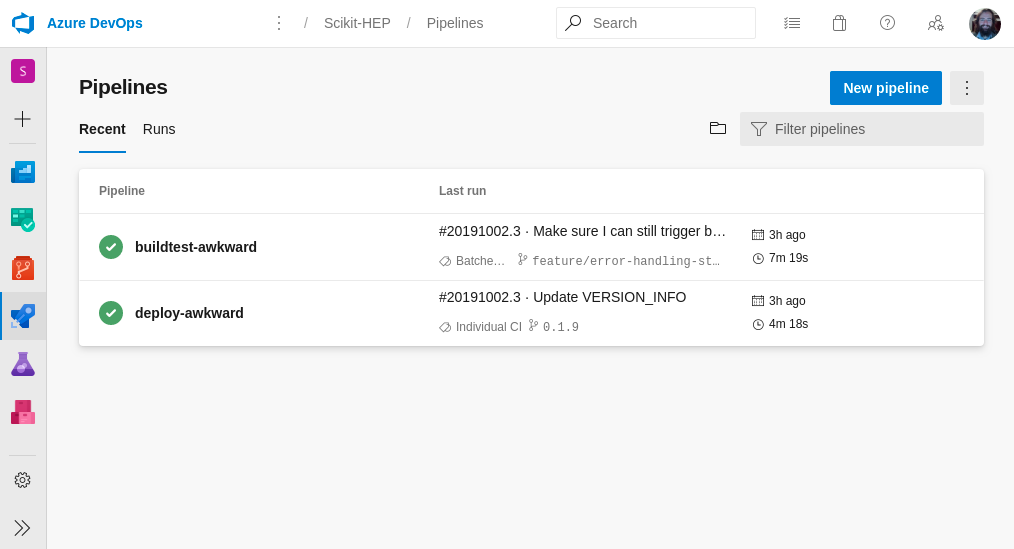
\includegraphics[width=\linewidth]{azure-screenshot.png}
\end{columns}
\end{frame}

\begin{frame}{Possibility of remote pair-programming: Atom Teletype}
\vspace{0.05 cm}
\begin{center}
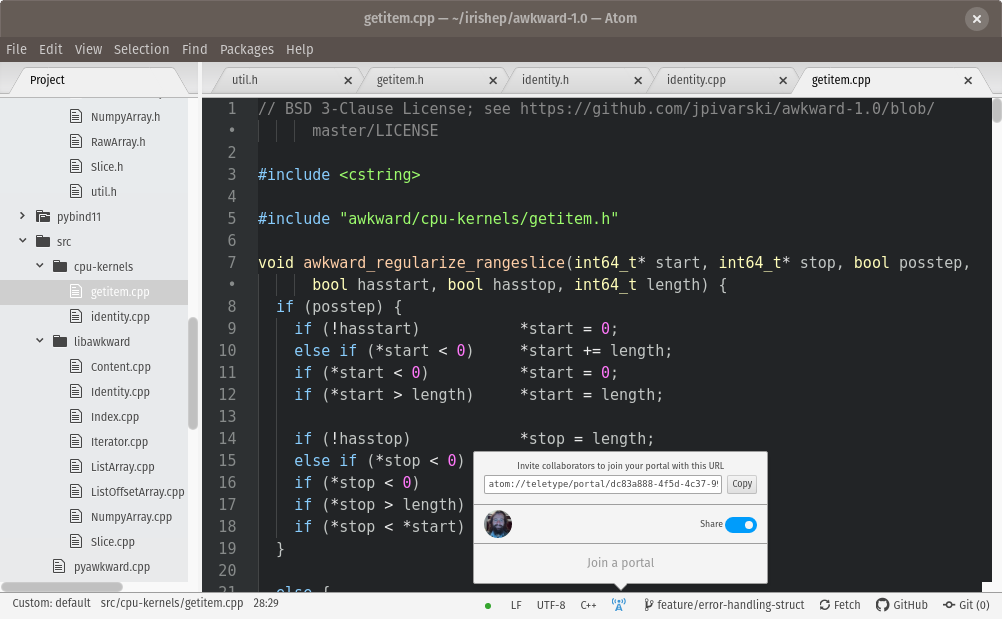
\includegraphics[width=0.9\linewidth]{atom-teletype.png}
\end{center}
\end{frame}

\begin{frame}{I've been developing in squash-and-merge pull requests}
\vspace{0.25 cm}
\tiny
\begin{columns}
\column{0.05\linewidth}
\column{0.95\linewidth}
\begin{itemize}
\item[\textcolor{darkblue}{2019-08-17}] set up a build process for the four layers with continuous deployment to Linux, MacOS, and Windows wheels.
\item[\textcolor{darkblue}{2019-08-22 (PR \href{https://github.com/scikit-hep/awkward-1.0/pull/2}{\#2})}] created a basic \mintinline{c++}{NumpyArray} and \mintinline{c++}{ListOffsetArray} in C++, exposed to Python with pybind11, and ensured correct memory management between Python's reference counts and C++'s \mintinline{c++}{std::shared_ptr}.
\item[\textcolor{darkblue}{2019-08-26 (PR \href{https://github.com/scikit-hep/awkward-1.0/pull/3}{\#3})}] extended Numba so that \mintinline{c++}{NumpyArray} and \mintinline{c++}{ListOffsetArray} can be used in Numba-compiled functions, ensuring no memory leaks/double frees.
\item[\textcolor{darkblue}{2019-08-27 (PR \href{https://github.com/scikit-hep/awkward-1.0/pull/4}{\#4})}] introduced \mintinline{c++}{Identity}, an optional surrogate key whose use is illustrated in \href{https://github.com/jpivarski/PartiQL\#readme}{PartiQL}.
\item[\textcolor{darkblue}{2019-08-29 (PR \href{https://github.com/scikit-hep/awkward-1.0/pull/5}{\#5})}] extended Numba to use \mintinline{c++}{Identity} as well, ensuring no memory leaks/double frees.
\item[\textcolor{darkblue}{2019-08-30 (PR \href{https://github.com/scikit-hep/awkward-1.0/pull/6}{\#6})}] added iteration to both C++ and Numba, as well as the first "operation," \mintinline{c++}{awkward1.tolist}, which turns an awkward array into Python lists (and eventually dicts, etc.).
\item[\textcolor{darkblue}{2019-09-02 (PR \href{https://github.com/scikit-hep/awkward-1.0/pull/7}{\#7})}] refactored \mintinline{c++}{Index}, \mintinline{c++}{Identity}, and \mintinline{c++}{ListOffsetArray} (and any other array types with \mintinline{c++}{Index}, which is nearly all of them) to have a 32-bit and a 64-bit version. My original plan to only support 64-bit in "chunked arrays" with 32-bit everywhere else is hereby scrapped—both bit widths will be supported on all indexes. Non-native endian, non-trivial strides, and multidimensional \mintinline{c++}{Index}/\mintinline{c++}{Identity} are not supported, though all of these features are allowed for \mintinline{c++}{NumpyArray} (which is {\it content}, not an {\it index}). The only limitation on \mintinline{c++}{NumpyArray} is that data must be C-ordered, not Fortran-ordered.
\item[\textcolor{darkblue}{2019-09-21 (PR \href{https://github.com/scikit-hep/awkward-1.0/pull/8}{\#8})}] C++ NumpyArray::getitem is done, setting the pattern for other classes (external C functions). The Numba and Identity extensions are not done, which would be necessary to fully set the pattern. This involved a lot of investigation (see [studies/getitem.py](https://github.com/jpivarski/awkward-1.0/blob/master/studies/getitem.py)).
\item[\textcolor{darkblue}{2019-09-21 (PR \href{https://github.com/scikit-hep/awkward-1.0/pull/9}{\#9})}] \mintinline{c++}{Identity} is correctly passed through \mintinline{c++}{NumpyArray} slices and \mintinline{c++}{__getitem__} uses \mintinline{c++}{get}, \mintinline{c++}{slice}, or the full \mintinline{c++}{getitem}, depending on argument complexity.
\item[\textcolor{darkblue}{2019-09-26 (PR \href{https://github.com/scikit-hep/awkward-1.0/pull/11}{\#11})}] fully implemented \mintinline{c++}{ListArray} and \mintinline{c++}{ListOffsetArray}'s \mintinline{c++}{__getitem__}.
\item[\textcolor{darkblue}{2019-10-02 (PR \href{https://github.com/scikit-hep/awkward-1.0/pull/12}{\#12})}] implemented \mintinline{c++}{ListArray.__getitem__(array)} in Numba, setting the pattern for all the other cases.
\end{itemize}
\end{columns}

\normalsize
\vspace{0.35 cm}
Mostly one commit per PR, which is one feature (except for fixing deployment bugs).
\end{frame}

\begin{frame}{Roadmap/Goals}
\Large
\begin{center}
Provide some minimally testable product this month \\ \textcolor{gray}{(for Coffea and thrill-seekers)}.

\vspace{1 cm}
Minimally usable for physics analysis in ``early 2020.''

\vspace{1 cm}
\end{center}

Start an {\normalsize \mintinline{python}{import awkward}} $\to$ {\normalsize \mintinline{python}{import awkward0}} \\
\phantom{Start an} {\normalsize \mintinline{python}{import awkward1}} $\to$ {\normalsize \mintinline{python}{import awkward}} transition by spring.
\end{frame}

\end{document}
